\documentclass{report}

\usepackage{booktabs}
\usepackage[utf8]{inputenc}
\usepackage{graphicx}
\usepackage{pgfplots}
\usepackage[l3]{csvsimple}
\DeclareUnicodeCharacter{2212}{−}
\usepgfplotslibrary{groupplots,dateplot}
\usetikzlibrary{patterns,shapes.arrows}
\pgfplotsset{compat=newest}

\title{MATH 610 PA 2 Report}
\author{Jordan Hoffart}
\date{}
\begin{document}
\maketitle

\chapter*{Problem 1}
\section*{Solution}
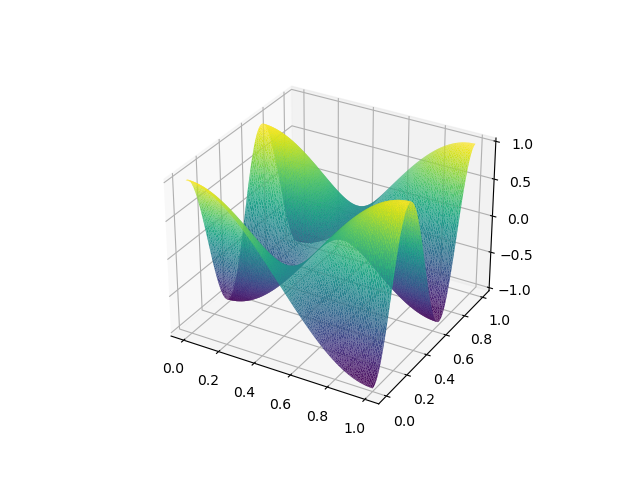
\includegraphics[width=\textwidth]{../data/problem-1/problem_1_plot.png}

\section*{Errors}
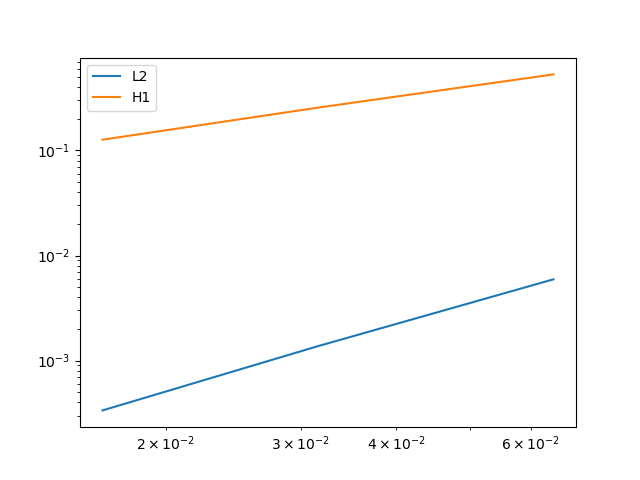
\includegraphics[width=\textwidth]{../data/problem-1/problem_1_errors.png}

\csvautotabular{../data/problem-1/problem_1_errors.csv}

\chapter*{Problem 2}
\section*{$q=1$}
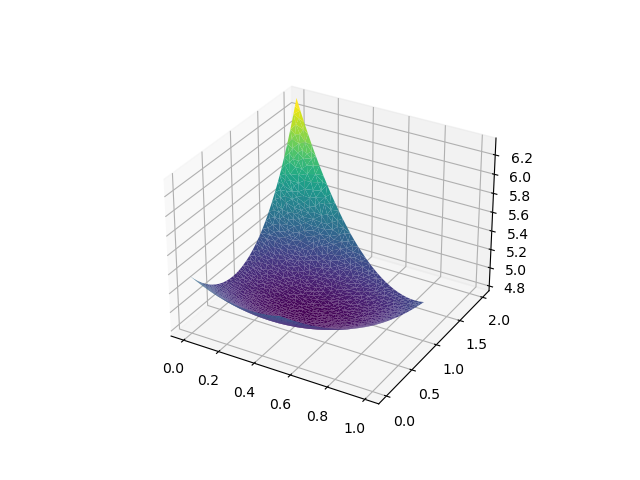
\includegraphics[width=\textwidth]{../data/problem-2/problem_2_q_1_plot_0.png}

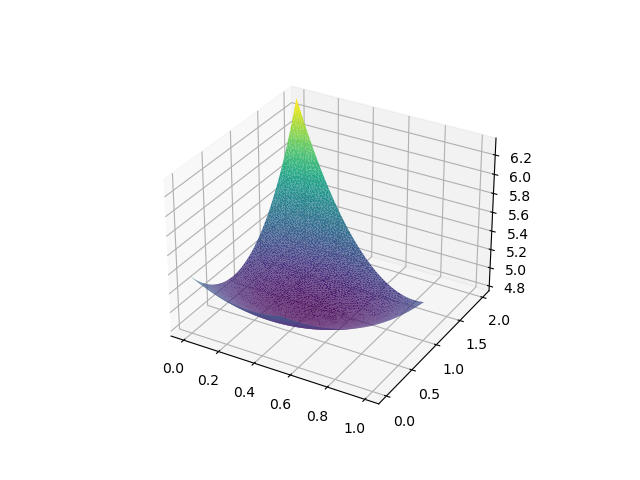
\includegraphics[width=\textwidth]{../data/problem-2/problem_2_q_1_plot_1.png}

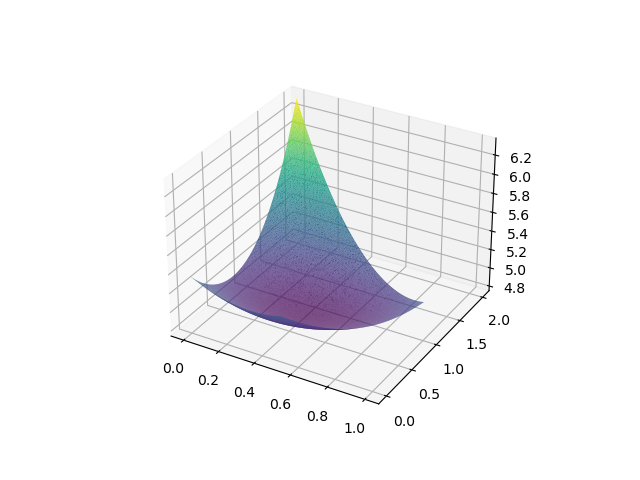
\includegraphics[width=\textwidth]{../data/problem-2/problem_2_q_1_plot_2.png}

\section*{$q=0$}
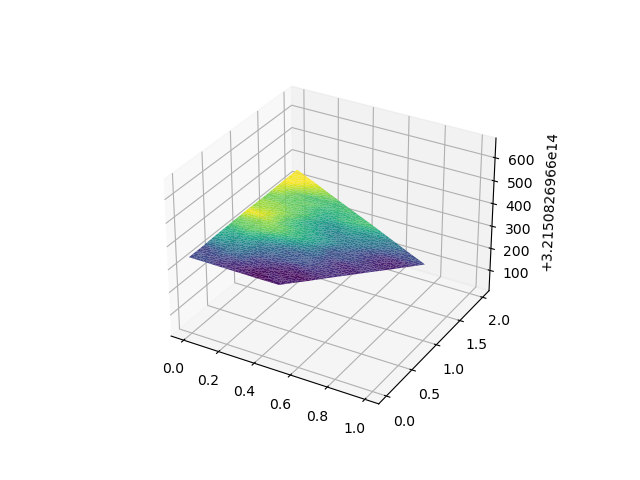
\includegraphics[width=\textwidth]{../data/problem-2/problem_2_q_0_plot_0.png}

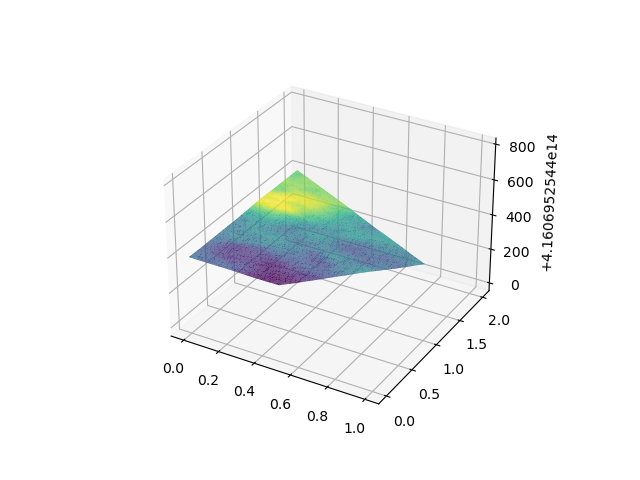
\includegraphics[width=\textwidth]{../data/problem-2/problem_2_q_0_plot_1.png}

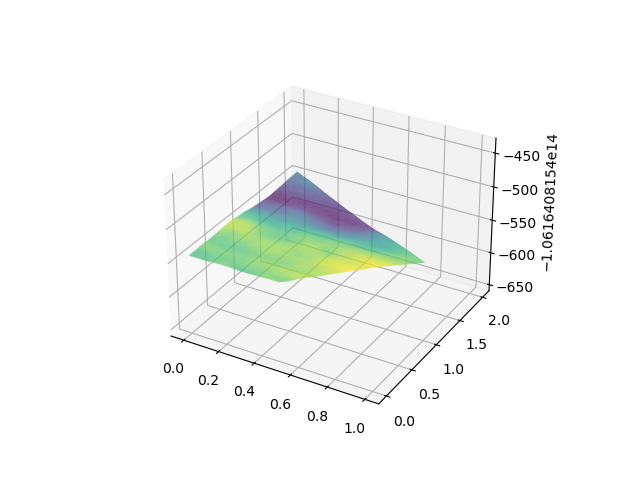
\includegraphics[width=\textwidth]{../data/problem-2/problem_2_q_0_plot_2.png}

\chapter*{Problem 3}
\section*{Manufactured solution}
\[u(x,y) = \cos(\pi x)\cos(3\pi y)\]
\subsection*{Solution}
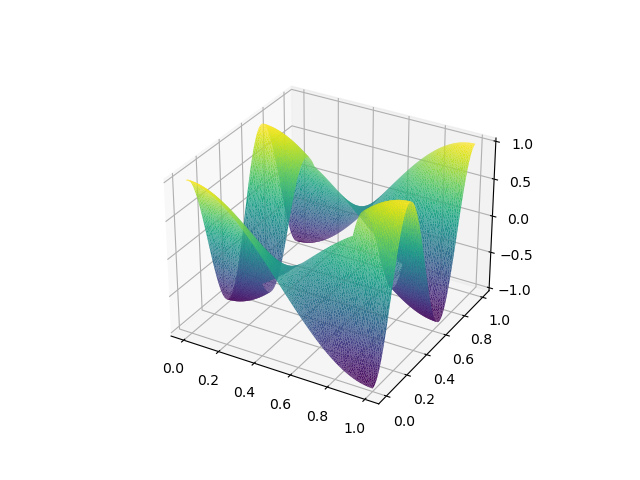
\includegraphics[width=\textwidth]{../data/problem-3/problem_3_manufactured.png}

\subsection*{Errors}
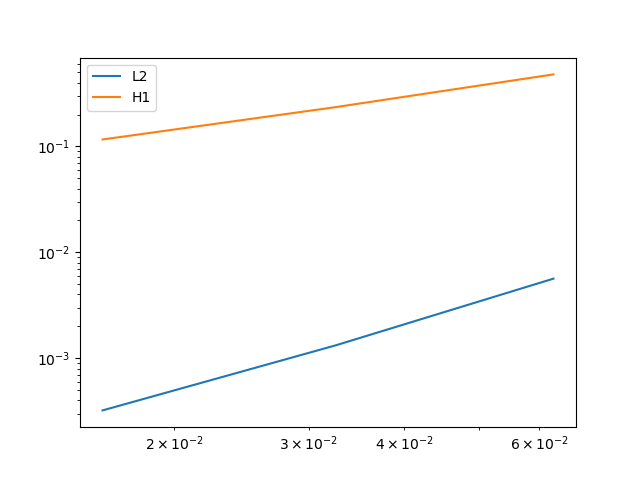
\includegraphics[width=\textwidth]{../data/problem-3/problem_3_manufactured_errors.png}

\csvautotabular{../data/problem-3/problem_3_errors.csv}

\section*{Unknown solution}
\subsection*{Solution}
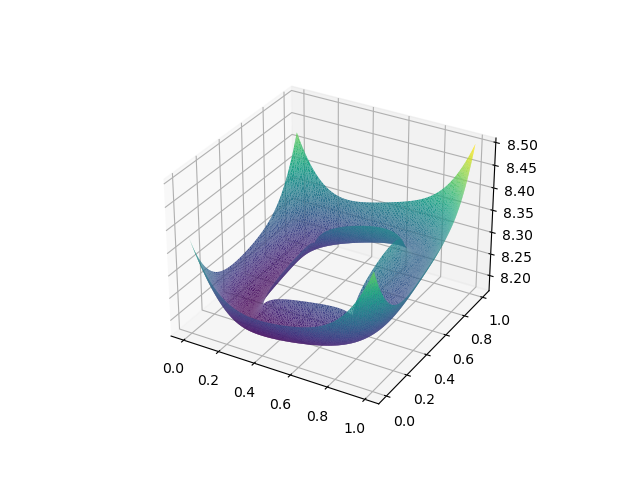
\includegraphics[width=\textwidth]{../data/problem-3/problem_3_plot.png}
\end{document}
